The digital components layer will consist of 4 devices. The first is a Raspberry
PI. This will act as the main computer of the system. It will the majority of
the data both from the server, the UI, and the microcontrollers. The other 3
components will all be ESP32 microcontrollers, but they will each serve a
different purpose. An ESP32 will receive information from a thermometer sensor
and relay it to the heat control ESP32. Based on what the temperature is, the
heat control ESP32 will trigger the relay to activate or deactivate the heating
element. The final ESP32 will be used to trigger the relay to turn on the pump
based on what the message broker instructs it to do.   

\begin{figure}[h!]
	\centering
 	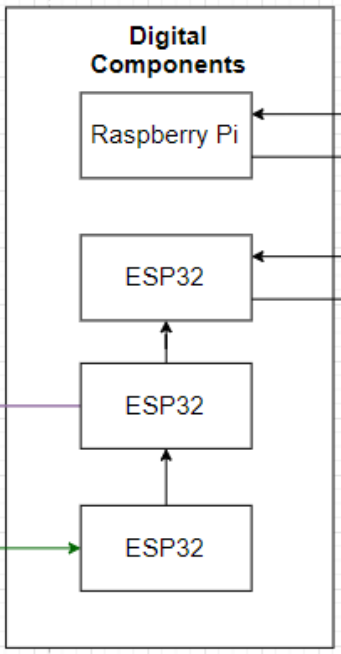
\includegraphics[width=0.30\textwidth]{images/digital_components.png}
  \caption{Digital Components Subsystem}
\end{figure}

\subsection{Digital Components Layer Hardware}
The hardware used in the digital components subsystem will made up of two
different types of electronics. The computer that acts as the arbiter of tasks
will be a Raspberry Pi 3b+. The microcontrollers used are ESP32s. 

\subsection{Digital Components Layer Operating System}
The Raspberry Pi 3b+ will run Raspbian OS. There will not be an operating system
on the microcontrollers. 

\subsection{Raspberry Pi Subsystem}
The Raspberry PI will host the web server and the MQTT client. The RBP will
receive information from the web server about what the user inputed via the UI.
It will then take that information and relay it to the microcontrollers using
the MQTT protocol. The RBP will then receive sensor data from the
microcontrollers through MQTT messages and send store the information in the web
server. 

\subsubsection{Subsystem Hardware}
The hardware involved in this layer will consist only of a Raspberry Pi 3b+.

\subsubsection{Subsystem Operating System}
The operating system used will be Raspbian OS.

\subsubsection{Subsystem Software Dependencies}
This subsystem will use the Mosquitto MQTT Message Broker. 

\subsubsection{Subsystem Programming Languages}
This subsystem will at the most use a scripting language such as BASH. 

\subsection{Temperature Sensor Subsystem}
The microcontroller will await messages from the message broker. The message
broker will recieve information from the thermometer ESP32. If the temperature
is too low, the message broker will send a message to this microcontroller to
trigger the relay and allow power to flow to the heating element. If the
temperature gets too high on the heating element, the message broker will tell
this microcontroller to deactivate the heating element.

\subsubsection{Subsystem Hardware}
The hardware involved in this layer will consist of a microcontroller ESP32 and a temperature
sensor MAX6675. 

\subsubsection{Subsystem Operating System}
None will be used for this subsystem.

\subsubsection{Subsystem Software Dependencies}
Arduino libraries will be used for the temperature sensor. 

\subsubsection{Subsystem Programming Languages}
C++ will be used to program the ESP32.

\subsubsection{Subsystem Data Structures}
The ESP32 will read data from the temperature sensor, and send it to the
Raspberry Pi for a decision to be made. The data will be passed via the MQTT protocol.

\subsection{Heat Control Subsystem}
The microcontroller will await messages from the message broker. The message
broker will recieve information from the thermometer ESP32. If the temperature
is too low, the message broker will send a message to this microcontroller to
trigger the relay and allow power to flow to the heating element. If the
temperature gets too high on the heating element, the message broker will tell
this microcontroller to deactivate the heating element.

\subsubsection{Subsystem Hardware}
The hardware involved will be an ESP32 and a 120V heating element. 

\subsubsection{Subsystem Operating System}
None will be used for this subsystem.

\subsubsection{Subsystem Software Dependencies}
Arduino MQTT libraries for the ESP32.

\subsubsection{Subsystem Programming Languages}
C++ will be used to program the ESP32.

\subsubsection{Subsystem Data Structures}
Commands will be sent to the ESP32 via MQTT messages. 

\subsection{Pump Control Subsystem}
This microcontroller will await messages from the message broker. When the
message broker sends it the message to turn on the pump, the microcontroller
will trigger the relay to allow power to go to the pump. When the message broker
sends the message to turn off the pump, the microcontroller will cease sending
power to the relay, causing it to close, and power will not be supplied to the
pump.

\subsubsection{Subsystem Hardware}
The hardware for this subsystem will consist of a single ESP32.

\subsubsection{Subsystem Operating System}
None will be used for this subsystem. 

\subsubsection{Subsystem Software Dependencies}
Arduino MQTT libraries for the ESP32.

\subsubsection{Subsystem Programming Languages}
C++ will be used to program the ESP32.

\subsubsection{Subsystem Data Structures}
Commands will be sent to the ESP32 via MQTT messages. 
